\documentclass[utf8,compress]{beamer}

\usetheme{Warsaw}

\usepackage[francais]{babel}

\newcommand{\slidesubject}{Présentation en \LaTeX}

\title{Exemple}
\subtitle{\slidesubject}
\subject{\slidesubject}
\author{Bruno \textsc{Voisin}}
\institute{
    Université de \LaTeX\\
    Entreprise\\
    \vspace{0.8em}
    \emph{- Responsables -} \\
    M.~Maitre \textsc{Destage}\\
    M.~En \textsc{Cadran}
}
\date{01 juillet 2012}

%% Définition du répertoire contenant les images
\graphicspath{{images/}}

\logo{
\includegraphics[height=1cm]{LaTeX-logo.png}}

%% Numérotation des slides :
%% http://texblog.net/latex-archive/plaintex/beamer-footline-frame-number/

%% Solution 1
%\newcommand*\oldmacro{}%
%\let\oldmacro\insertshorttitle%
%\renewcommand*\insertshorttitle{%
%  \oldmacro\hfill%
%  \insertframenumber\,/\,\inserttotalframenumber}

%% Solution 2
\expandafter\def\expandafter\insertshorttitle\expandafter{%
  \insertshorttitle\hfill%
  \insertframenumber}

\begin{document}

\begin{frame}
\titlepage
\end{frame}

\logo{
\includegraphics[height=1cm]{LaTeX-logo-transp25.png}}


\section{Introduction}

\begin{frame}{Introduction}
\begin{block}{C'est quoi ce document ?}
    Ce document est un exemple de présentation (sous forme de diapositives) faite en LaTeX.
\end{block}
\begin{block}{Où trouver les sources ?}
    Les sources sont disponibles sur mon blog \url{http://blog.hikoweb.net/}.
\end{block}
\begin{block}{Je peux m'en inspirer pour ma propre présentation ?}
    Oui, vous êtes libre d'utiliser les sources comme bon vous semble.
\end{block}
\end{frame}

\begin{frame}{Plan}
\tableofcontents
\end{frame}

%% Un rappel du plan sera affiché à chaque début de section.
\AtBeginSection[]
{
  \begin{frame}<beamer>
    \frametitle{Plan}
    \tableofcontents[currentsection]
  \end{frame}
}


\section{Première section}

\subsection{Une sous-section}

\begin{frame}{La page la plus simple}
C'est simple, il n'y a que du texte.

Quae feminas feminas poterat pedibus ter quocumque nixus usque usque oculos exprimunt nixus quocumque tergentes iactari nixus taedium simulacra tergentes.
\end{frame}

\begin{frame}[containsverbatim]{Les blocs}
\begin{block}{Bloc normal}
     C'est un joli bloc bleu.
\end{block}
\begin{exampleblock}{Bloc exemple}
     Le vert signifie que c'est un exemple.
\end{exampleblock}
\begin{alertblock}{Bloc alerte}
     Attention c'est rouge !
\end{alertblock}
\end{frame}

\subsection{Une autre sous-section}

\begin{frame}{Juste une image}
\begin{figure}[h]
    \center
    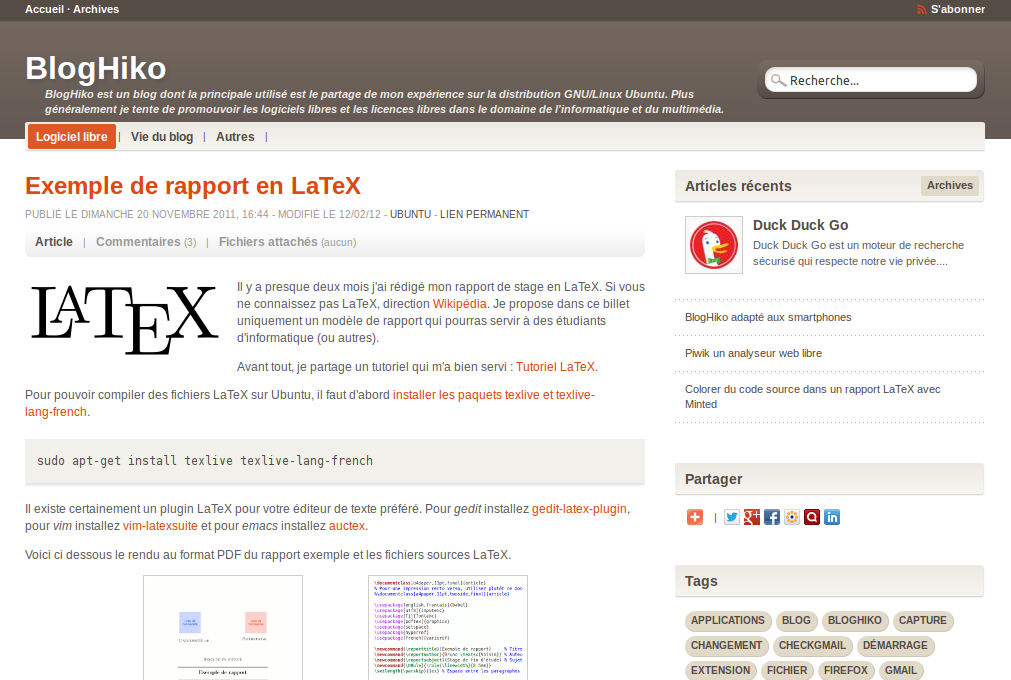
\includegraphics[width=\textwidth]{bloghiko.png}
\end{figure}
\end{frame}


\section{Deuxième section}

\subsection{C'est pas fini}

\begin{frame}{Liste}
\begin{itemize}
    \item Une simple liste,
    \item avec deux éléments.
\end{itemize}
\begin{block}{Implication}
    \begin{itemize}
    \item cause
    \item[$\Rightarrow$] conséquence
    \end{itemize}
\end{block}
\end{frame}

\begin{frame}{Plus compliqué}
\begin{columns}
\begin{column}{0.7\textwidth}
    Cette page est constituée de\dots
    \begin{itemize}
    \item deux colonnes ;
    \item un liste dans la première colonne ;
    \item une image dans la deuxième colonne ;
    \item un bloc.
    \end{itemize}
\end{column}
\begin{column}{0.3\textwidth}
    \begin{figure}[h]
        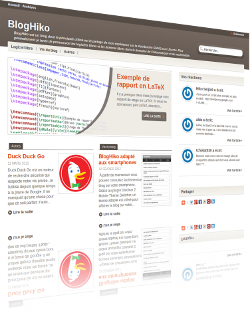
\includegraphics[width=3cm]{bloghiko-reflet3d.png}
    \end{figure}
\end{column}
\end{columns}
\vspace{1em}
\begin{block}{Le bloc}
    Ut eum praeceptum possemus fuit diligendo aliquando diligentiam ut 
    fuit hoc quam inimicitiarum possemus praeceptum.
\end{block}
\end{frame}


\section{Conclusion}

\begin{frame}{Conclusion}
    Vous pouvez faire des diapositives très professionnelles en toute simplicité.
\end{frame}

\end{document}

